\documentclass[landscape,a0paper,fontscale=0.34]{baposter}
\usepackage{amssymb}
\usepackage{amsmath}
\usepackage{amsthm}
%\usepackage{amsaddr} % to allow inclusion of institution address
%\usepackage{charter}
\usepackage{enumitem}
%\usepackage{wrapfig}
\usepackage{caption}
\usepackage{floatrow}  % to place graph and caption side by side
\usepackage{multicol}
\usepackage{listings}
\usepackage{tikz}
\usepackage{url}
% packages for the table
\usepackage{booktabs}
\usepackage{longtable}
\usepackage{array}
\usepackage{multirow}
\usepackage{wrapfig}
\usepackage{float}
\usepackage{colortbl}
\usepackage{pdflscape}
\usepackage{tabu}
\usepackage{threeparttable}
\usepackage{threeparttablex}
\usepackage[normalem]{ulem}
\usepackage{makecell}
\usepackage{xcolor}



%\usepackage{tikz}
%\usepackage{tkz-graph}

%\usepackage{subcaption} % for better subcaptions
%\usepackage{verbatim}   % for comment environment
%\usepackage{booktabs}   % for publication-quality tables
%\usepackage{algorithm}  % for the algorithm environment
%\usepackage[flushleft, online]{threeparttable} % for table footnotes
%\usepackage{grffile}

%\usepackage[usenames,dvipsnames]{color} % for highlighting / strikethroughs
%\usepackage{multicol}
\definecolor{boxcolour}{RGB}{120,245,230}
\definecolor{boxcolour}{RGB}{191, 250, 238}
\definecolor{UCLABlue}{RGB}{39,116,174}
\definecolor{boxcolour}{RGB}{39,116,174}


%%%%%%%%%%%%%%%%%%%%%%%%%%%%%%%%%%%%%%%%%%%%%%%%%%%%%%%%%%%%%%%%%%%%%%%%%%%%%%%%
% Multicol Settings
%%%%%%%%%%%%%%%%%%%%%%%%%%%%%%%%%%%%%%%%%%%%%%%%%%%%%%%%%%%%%%%%%%%%%%%%%%%%%%%%
\setlength{\columnsep}{0.7em}
\setlength{\columnseprule}{0mm}

%%%%%%%%%%%%%%%%%%%%%%%%%%%%%%%%%%%%%%%%%%%%%%%%%%%%%%%%%%%%%%%%%%%%%%%%%%%%%%%%
% Save space in lists. Use this after the opening of the list
%%%%%%%%%%%%%%%%%%%%%%%%%%%%%%%%%%%%%%%%%%%%%%%%%%%%%%%%%%%%%%%%%%%%%%%%%%%%%%%%
\newcommand{\xcompresslist}{%
 \setlength{\itemsep}{1pt}%
 \setlength{\parskip}{0pt}%
 \setlength{\parsep}{0pt}%
}

\newcommand{\compresslist}{%
 \setlength{\itemsep}{5pt}%
 \setlength{\parskip}{0pt}%
 \setlength{\parsep}{0pt}%
}

\newcommand{\compresslistless}{%
 \setlength{\itemsep}{3.25pt}%
 \setlength{\parskip}{0pt}%
 \setlength{\parsep}{0pt}%
}

%Special for paper
\def\phi{\varphi}
\def\by{\mathbf{y}}
\def\bs{\mathbf{\sigma}}
\def\bX{\mathbf{X}}
\def\bB{\mathbf{B}}
\def\bPhi{\mathbf{\Phi}}
\def\brho{\mathbf{\rho}}
\def\pl{p_\lambda}
\def\pln{p_{\lambda_n}}
\def\G{\mathcal{G}}
\def\rto{\leftarrow}
\def\s{\sigma}
\def\o{\omega}
\def\A{\mathcal{A}}
\renewcommand{\th}{\theta}
%\renewcommand{\thh}{\hat{\theta}}
\newcommand{\bth}{\boldsymbol\theta}
\renewcommand{\b}{\beta}
\newcommand{\hb}{\hat{\beta}}
\newcommand{\hbB}{\widehat{\mathbf{B}}}
\newcommand{\hB}{\widehat{B}}
\newcommand{\hO}{\widehat{\Omega}}
\newcommand{\hP}{\widehat{\Phi}}
\newcommand{\hR}{\widehat{R}}
\newcommand{\hT}{\widehat{\Theta}}
\newcommand{\one}{\mathbf{1}}
\def\bn{\boldsymbol\nu}
\def\bu{\mathbf{u}}
\newcommand{\tB}[1]{\widetilde{B}(#1)}
\newcommand{\tOm}[1]{\widetilde{\Omega}(#1)}

%%%%%%%%%%%%%%
\def\estperm{\widehat{\pi}}
\def\dagadjest{\widehat{B}}
\def\goodperm{\pi_{0}}
\def\penderiv{\rho_\lambda'(0+)}

% defining new colors for text
\definecolor{test}{rgb}{0,50,0}
\newcommand{\cemph}[1]{\textcolor{cyan!80!blue}{#1}}
\newcommand{\ccemph}[1]{\textcolor{magenta}{#1}}

%%%%%%%%%%%%%%%%%%%%%%%%%%%%%%%%%%%%%%%%%%%%%%%%%%%%%%%%%%%%%%%%%%%%%%%%%%%%%
%% Begin of Document
%%%%%%%%%%%%%%%%%%%%%%%%%%%%%%%%%%%%%%%%%%%%%%%%%%%%%%%%%%%%%%%%%%%%%%%%%%%%%
\begin{document}
%%%%%%%%%%%%%%%%%%%%%%%%%%%%%%%%%%%%%%%%%%%%%%%%%%%%%%%%%%%%%%%%%%%%%%%%%%%%%
%% Here starts the poster
%%---------------------------------------------------------------------------
%% Format it to your taste with the options
%%%%%%%%%%%%%%%%%%%%%%%%%%%%%%%%%%%%%%%%%%%%%%%%%%%%%%%%%%%%%%%%%%%%%%%%%%%%%
\begin{poster}{
 % Show grid to help with alignment
 grid=false,
 columns=3,
 % Column spacing
 colspacing=1em,
 % Color style
 headerColorOne=boxcolour, %gray!20!white!90!black,
 borderColor=boxcolour,
 % Format of textbox
 textborder=rectangle,
 linewidth=0.25mm,
 % Format of text header
 headerborder=closed,
 headershape=rectangle,
 headershade=plain,
 headerfont=\large\rmfamily\bf,
 background=none,
 bgColorOne=gray!90!black,
 boxColorOne=white,
 headerheight=0.12\textheight}
 % Eye Catcher
 {
  \begin{tabular}{c}
    
\includegraphics[height=2cm, width = 8cm]{globe.jpg}%{ucla_cw}
  \end{tabular}
 }
 % Title
 {\huge \centering GLOBE Research: Leadership and Societal Perspectives}
 % Authors
{\vspace{0.2cm} Ethan Allavarpu $\cdot$ Raymond Bai $\cdot$ Jaclyn Chiu $\cdot$ Ariel Chow $\cdot$ Carlie Lin $\cdot$ Dara Tan \\ \vspace{0.2cm} \large GitHub Repository: \url{https://github.com/ethan-allavarpu/stats140-final}}
 % University logo
 {
  \begin{tabular}{c}
    
\includegraphics[height=2cm, width = 8cm]{ps_statistics_DoS} %{ucla_cw}
  \end{tabular}
 }
%%%%%%%%%%%%%%%%%%%%%%%%%%%%%%%%%%%%%%%%%%%%%%%%%%%%%%%%%%%%%%%%%%%%%%%%%%%%%%
%%% Now define the boxes that make up the poster
%%%---------------------------------------------------------------------------
%%% Each box has a name and can be placed absolutely or relatively.
%%% The only inconvenience is that you can only specify a relative position
%%% towards an already declared box. So if you have a box attached to the
%%% bottom, one to the top and a third one which should be inbetween, you
%%% have to specify the top and bottom boxes before you specify the middle
%%% box.
%%%%%%%%%%%%%%%%%%%%%%%%%%%%%%%%%%%%%%%%%%%%%%%%%%%%%%%%%%%%%%%%%%%%%%%%%%%%%%

%%%%%%%%%%%%%%%%%%%%%%%%%%%%%%%%%%%%%%%%%%%%%%%%%%%%%%%%%%%%%%%%%%%%%%%%%%%%%%
\headerbox{\color{white}Background}{name=background,column=0,row=0,span=1}{
	The GLOBE (Global Leadership \& Organizational Behavior Effectiveness) research program is an interdisciplinary study aiming to identify the interrelationships between societal culture, societal effectiveness and organizational leadership. Surveying from over 17,000 middle managers from 62 cultures, the 2004 research survey provides data that measures the leadership and societal culture practices of each country (House et al, 2004). The data appear on a scale from 1 to 7.

	%The analysis concerns the 2004 research survey data from the Global Leadership \& Organizational Behavior Effectiveness (GLOBE) project. The project surveyed from over 1,000 CEOs and over 5,000 senior executives in corporations in a variety of industries in 24 countries (This is from GLOBE study of 2014), with the motivation of identifying interrelationships between societal culture, societal effectiveness and organizational leadership.%

}

\headerbox{\color{white}Exploratory Data Analysis}{name=eda,column=0,row=0,span=1, below = background}{
	When looking at the leadership data, the correlations between different variables tended to aggregate into groups, leading us to consider \textit{how many} of these groups existed and whether countries viewed them similarly.

	For the societal characteristics, we noticed two types of characteristics: societal \textit{values} and societal \textit{practices}. We used scatterplots to visualize the relationship between these two variables:
	\begin{center}
	    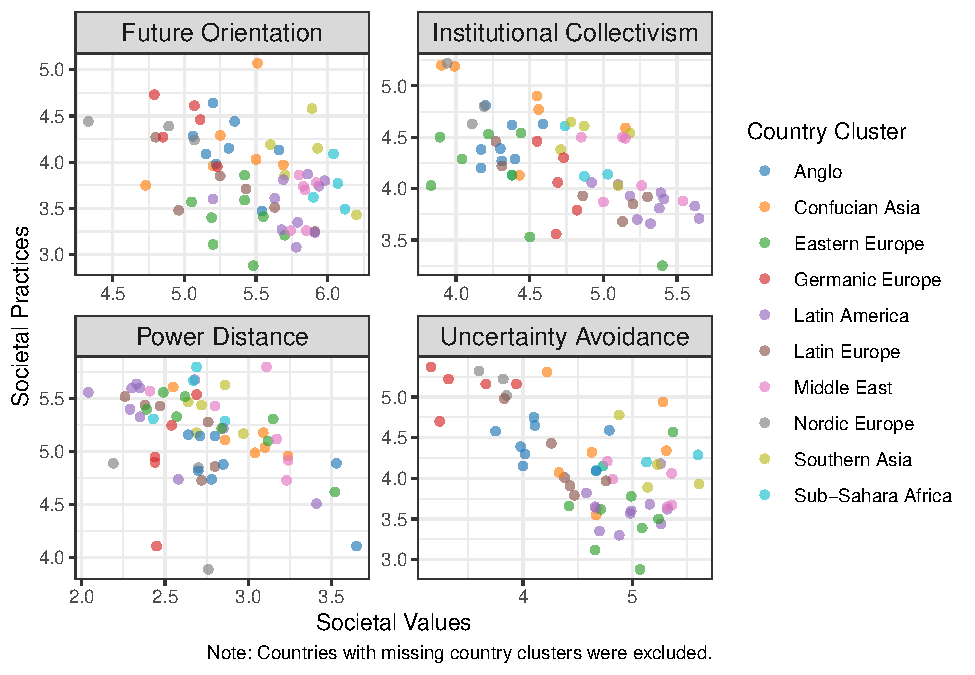
\includegraphics[scale = 0.65]{SPV Plots-1.pdf}
	\end{center}
	From the above examples, we saw that the practices and values did not necessarily align, prompting us to further investigate these relationships.
}

\headerbox{\color{white}Research Questions}{name=problem,column=0,row=0,span=1, below = eda}{
	\xcompresslist
	\begin{enumerate}
		\setlength{\itemsep}{1pt}
        \setlength{\parskip}{0pt}
        \setlength{\parsep}{0pt}
		\item Which characteristics or traits do countries tend to group together when determining "good" leadership values?
		\item Do societal practices and societal values align? If they do not, which practices and values deviate the most significantly?
	\end{enumerate}
}

%%%%%%%%%%%%%%%%%%%%%%%%%%%%%%%%%%%%%%%%%%%%%%%%%%%%%%%%%%%%%%%%%%%%%%%%%%%%%%
\headerbox{\color{white}Analysis Methodology}{name=method, column=0, row=2, span=1, below=problem}{
%\begin{wrapfigure}{r}{4cm}
%\end{wrapfigure}
(1) For the analysis of leadership qualities, we first performed principal component analysis (PCA) to dimension-reduce the existing leadership value variables into major principal components that capture most variability in the data. Using $k$-means clustering, we separated the leadership values into $k$ clusters such that there is minimal variance between data points belonging to the same cluster (minimal within-cluster variability) and high variance between any two clusters (high between-cluster variability). By mapping the leadership values corresponding to each country to the principal components, we can use the same clustering method to group countries by their similarities in valuation of leadership qualities.
}
\headerbox{\color{white}Analysis Methodology}{name=method2, column=1, row=0, span=1}{
(2) For the analysis of alignment between societal values and societal practices, we employed simple linear regression (SLR) models to predict their relationship.  We fit the model:
$$ y = \beta_{0} + \beta_{1}x$$
where $x$ is the societal values rating and $y$ is the societal practices rating for the nine cultural dimensions. Additionally, we performed t-tests for each dimension to test the null hypothesis that there is no relationship between the societal value and practice ($H_0: \beta_1 = 0$ versus $H_1: \beta_1 \neq 0$). We employed Bonferroni corrections to adjust the significance threshold from $\alpha = 0.05$ to $\alpha \approx 0.0056$.
}

\definecolor{clust3}{HTML}{408000BF}
\definecolor{clust2}{HTML}{800080BF}
\definecolor{clust1}{HTML}{008080BF}
\definecolor{clust4}{HTML}{739999BF}
\definecolor{clust5}{HTML}{000026BF}
\definecolor{clust6}{HTML}{407326BF}
\definecolor{clust7}{HTML}{BF7300BF}

\headerbox{\color{white}Analysis Results}{name=analysis,column=1, row=1, span=1, below=method2}{
	After performing PCA, we split the leadership values into $k = 3$ groups by clustering on the first four principal components:
	\begin{enumerate}[noitemsep]
	%remove [noitemsep] for more spacing among the colored list
	    \color{clust1}
	    \item Internally competitive, malevolent, status conscious, self-centred, bureaucratic, face saver, autocratic
	    \color{clust2}
	    \item Humane-oriented, modesty
	    \color{clust3}
	    \item Participative, team integrator, inspirational, autonomous, administratively competent, integrity, visionary, diplomatic, decisive, collaborative team orientation, self-sacrifice, performance-oriented
	\end{enumerate}
	\vspace{2mm}

	After looking at the clusters for the leadership characteristics, we considered which \textit{countries} had similar leadership perspectives. By transforming the leadership variables in each country to the first four principal components, we can then perform $k$-means clustering, yielding four distinct clusters colored in \color{clust4}light blue\color{black}, \color{clust5}dark blue\color{black}, \color{clust6}green\color{black}, and \color{clust7}gold\color{black}:
	\begin{center}
	    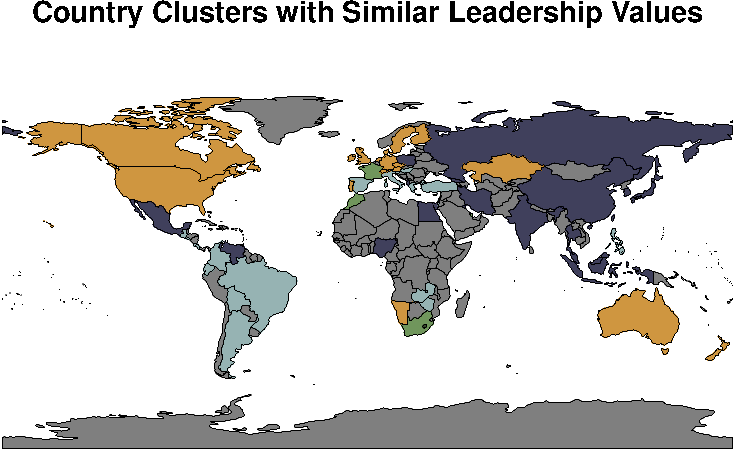
\includegraphics[scale=.07]{kmeans-1.pdf}
	\end{center}
	\color{black}
	\textit{Note: East and West Germany belong to the same cluster and are colored as such. South Africa is colored by the cluster the Black sample belongs in, rather than the White sample. Countries that are not included in the data are colored gray.}
    \vspace{2mm}

	The countries in each cluster align geographically (except for one). The gold region consists of western European and Anglo countries, light blue with Latin America and the Mediterranean, and dark blue with Asia. The only interesting development was the green cluster: there were only four countries (France, Morocco, South Africa (Black sample), and Qatar.
}

%%%%%%%%%%%%%%%%%%%%%%%%%%%%%%%%%%%%%%%%%%%%%%%%%%%%%%%%%%%%%%%%%%%%%%%%%%%%%%
\headerbox{\color{white}Analysis Results}{name=analysis2,column=2,span=1, row=0}{
The table below shows the values of $\beta_1$ that we obtained from our SLRs and the corresponding p-values. Cultural dimensions for which the p-value is lower than the corrected $\alpha \approx 0.0056$ are indicated with green shading.
\begin{center}
\begin{tabular}[t]{lrr}
\toprule
Cultural Dimension & Coefficient Value & p-value \\
\midrule
\cellcolor[HTML]{E5F5E0}{Uncertainty Avoidance} & \cellcolor[HTML]{E5F5E0}{-0.6199} & \cellcolor[HTML]{E5F5E0}{0.0000}\\
\cellcolor[HTML]{E5F5E0}{Institutional Collectivism} & \cellcolor[HTML]{E5F5E0}{-0.5251} & \cellcolor[HTML]{E5F5E0}{0.0000}\\
\cellcolor[HTML]{E5F5E0}{Power Distance} & \cellcolor[HTML]{E5F5E0}{-0.4991} & \cellcolor[HTML]{E5F5E0}{0.0006}\\
\cellcolor[HTML]{E5F5E0}{Future Orientation} & \cellcolor[HTML]{E5F5E0}{-0.4725} & \cellcolor[HTML]{E5F5E0}{0.0009}\\
Humane Orientation & -0.5944 & 0.0116\\
\cellcolor[HTML]{F0F0F0}{Gender Egalitarianism} & \cellcolor[HTML]{F0F0F0}{0.2437} & \cellcolor[HTML]{F0F0F0}{0.0124}\\
Performance Orientation & -0.3459 & 0.0268\\
\cellcolor[HTML]{F0F0F0}{Assertiveness} & \cellcolor[HTML]{F0F0F0}{-0.1507} & \cellcolor[HTML]{F0F0F0}{0.0414}\\
In-group Collectivism & 0.4393 & 0.0991\\
\bottomrule
\end{tabular}
\end{center}

Most of the $\beta_1$ values are negative, including all four values that are significant at the $\alpha \approx 0.56$\% significant level as calculated using the Bonferroni correction.
}

\headerbox{\color{white}Conclusion}{name=conclusion,column=2,span=1, row=1, below = analysis2}{
Leadership characteristics are largely clustered based on whether each trait is negative or positive. For example, the traits malevolent and self-centered have similar ratings while the traits integrity and inspiration also have similar ratings. Additionally, leadership values tend to be clustered based on their geographic region. This suggests countries within smaller distances of one another have more similar leadership perspectives.

\vspace{2mm}
Our findings indicate that the societal practices and values of countries do not align and are instead generally opposing. Thus, we conclude that a country's societal value does not entail the same practices exercised among its constituents. This analysis can be useful for government officials trying to develop policies that promote cultural values. If a country places a high value on uncertainty avoidance (the desire to rely on social norms and procedures to avoid unpredictable events), then the same country may undergo unexpected and unconventional events in the future.}

\headerbox{\color{white}Limitations and Further Research}{name=limitation,column=2,span=1, row=2, below = conclusion}{
In the dataset, there are only 62 cultures observed (some countries split in two), limiting the significance of the analysis and the confidence we have in clustering countries by geographical similarities. In addition, there is no explanation as to why only certain countries were surveyed. We also recognize that at the time of data collection, the Apartheid and the Berlin Wall potentially played significant factors in the differing valuations of social and leadership values for citizens in South Africa and Germany, respectively. For further research, we can investigate if other indices (such as freedom index, government approval ratings, or a happiness index) could help explain the groupings of clusters in the PCA analysis. Researchers should also look into the potential causes behind the inverse relationship between social values and practices.

%While the analysis results seem promising, there are a few issues with the data we need to consider. First, there are only 62 countries observed, limiting the significance of the analysis and the confidence we have in clustering countries by geographical similarities. In addition, there is no explanation as to why only certain countries were surveyed. We also recognize that at the time of data collection in 2006, the Apartheid and the Berlin Wall potentially played significant factors in the differing valuations of social and leadership values for citizens in South Africa and Germany, respectively. For both leadership and societal analysis, further research should be conducting more surveys to look at the potential changes in ideology and perspectives over time on both the national and global level. Furthermore, we can investigate if other indices (such as freedom index, government approval ratings, or a happiness index) could help explain the groupings of clusters in the PCA analysis. Future researchers should also look into the potential causes behind the inverse relationship between social values and practices.%
}


\headerbox{\color{white}References}{name=reference,column=2,span=1, below=limitation}{
\small
ISO Country Codes: \url{https://en.wikipedia.org/wiki/ISO_3166-1_alpha-3} \\
\emph{House, Robert J, et al., editors. Culture, Leadership, and Organizations the Globe Study of 62 Societies. SAGE Publications, 2004.}
}

\end{poster}%
\end{document}
